\documentclass[10pt]{article}
\usepackage[margin=1in]{geometry}
\usepackage{amsmath,amssymb,bm}
\usepackage{graphicx}
\usepackage{microtype}
\usepackage[hidelinks]{hyperref}
\usepackage[numbers,sort&compress]{natbib}
\usepackage{titlesec}
\usepackage{enumitem}
\linespread{0.92}
\setlist{nosep,leftmargin=*}
\titlespacing*{\section}{0pt}{0.72ex plus 0.2ex}{0.35ex}
\titlespacing*{\subsection}{0pt}{0.50ex plus 0.1ex}{0.25ex}
\titleformat{\section}{\normalsize\bfseries}{\thesection.}{0.4em}{}
\titleformat{\subsection}{\normalsize\bfseries}{\thesubsection.}{0.4em}{}
\setlength{\parindent}{0pt}
\setlength{\parskip}{2pt}
\setlength{\abovedisplayskip}{4pt}
\setlength{\belowdisplayskip}{4pt}
\setlength{\textfloatsep}{7pt}
\setlength{\floatsep}{6pt}
\setlength{\intextsep}{6pt}
\graphicspath{{figures/}}
\newcommand{\dd}{\mathrm{d}}
\newcommand{\cG}{\frac{8\pi G}{c^4}}
\newcommand{\Tmiss}{T^{\rm miss}_{\mu\nu}}
\newcommand{\Gobs}{G_{\mu\nu}[g^{\rm obs}]}
\newcommand{\Gbar}{G_{\mu\nu}[g^{\rm bar}]}

\title{Geometric Residuals and Weak-Field Warp Search in the Missing-Mass Problem}
\author{J. R. Landers}
\date{\vspace{-0.65em}May 2026}

\begin{document}
\maketitle
\vspace{-1.9em}

\begin{abstract}
This paper frames the dark matter / modified gravity problem as an inverse problem over spacetime-geometry residuals. The central comparison is between the metric predicted by general relativity from observed baryons and the effective metric implied by dynamics, lensing, and other observables. The discrepancy can be represented as a curvature residual, an effective missing stress-energy tensor, or, in the weak-field galactic limit, an acceleration or potential residual. Building on this formulation, a toy computational prototype searches directly over weak-field metric perturbations, or ``spacetime warps,'' instead of beginning with named theories such as NFW halos, MOND, or scalar-field dark matter. The experiments are synthetic and heuristic, but they demonstrate a useful workflow: infer the residual first, study what weak-field perturbations reproduce it, and only then ask what physical generator could produce such a residual.
\end{abstract}

\section{Motivation}

In general relativity, matter and curvature are tied by Einstein's equation,
\begin{equation}
G_{\mu\nu}[g]
=
R_{\mu\nu}[g]-\frac{1}{2}R[g]g_{\mu\nu}
=
\cG T_{\mu\nu}.
\end{equation}
Given an observed baryonic stress-energy tensor $T^{\rm bar}_{\mu\nu}$, ordinary general relativity predicts a baryonic metric $g^{\rm bar}_{\mu\nu}$ satisfying
\begin{equation}
\Gbar=\cG T^{\rm bar}_{\mu\nu}.
\end{equation}
However, galaxy rotation curves, galaxy-cluster dynamics, gravitational lensing, and cosmological structure formation suggest that the metric/potential structure inferred from observations does not generally match the field sourced by baryons alone. Flat spiral-galaxy rotation curves were an early central example \citep{Rubin1980}; modern mass models and rotation-curve surveys sharpen the discrepancy \citep{Lelli2016,McGaugh2016}.

The usual language is that there is ``missing mass.'' The residual language is slightly different: the observations imply a mismatch in the inferred metric or potentials. The problem is then to infer the latent physical generator, or mixture of generators, that produces that mismatch.

\section{Relativistic Residual}

Let $g^{\rm obs}_{\mu\nu}$ denote an effective spacetime metric inferred from the full set of observations. Formally define the Einstein-tensor residual
\begin{equation}
\boxed{
\Delta G_{\mu\nu}
:=
\Gobs-\Gbar .
}
\end{equation}
If the Einstein field equation is kept fixed, this residual defines an effective missing stress-energy tensor,
\begin{equation}
\boxed{
\Tmiss
:=
\frac{c^4}{8\pi G}\Delta G_{\mu\nu}.
}
\end{equation}
The ``missing stuff'' is whatever source term would have to be added to the baryonic stress-energy tensor so that the observed metric satisfies Einstein's equation:
\begin{equation}
G_{\mu\nu}[g^{\rm obs}]
=
\cG\left(T^{\rm bar}_{\mu\nu}+\Tmiss\right).
\end{equation}
If the residual is well modeled by a pressureless, weakly interacting component, then it resembles cold dark matter. In an idealized dust-like limit,
\begin{equation}
T^{\rm DM}_{\mu\nu}\approx \rho_{\rm DM}u_\mu u_\nu.
\end{equation}
But this is a hypothesis about the decomposition of the residual, not a mathematical necessity.

A modified-gravity interpretation instead moves part or all of the residual to the left-hand side:
\begin{equation}
G_{\mu\nu}[g]+\Delta{\cal E}_{\mu\nu}[g,T,\ldots]
=
\cG T^{\rm bar}_{\mu\nu}.
\end{equation}
Thus the core distinction is whether the residual is caused by missing stress-energy, missing field dynamics, baryonic modeling error, systematics, or a mixture of these.

\section{Weak-Field Galaxy Limit}

For disk galaxies the fields are weak and motions are nonrelativistic. A useful metric ansatz is
\begin{equation}
\dd s^2
\simeq
-\left(1+\frac{2\Phi}{c^2}\right)c^2\dd t^2
+
\left(1-\frac{2\Psi}{c^2}\right)\dd\mathbf{x}^2 .
\end{equation}
Nonrelativistic circular motion mainly probes $\Phi$:
\begin{equation}
v^2(r)=r\frac{\dd\Phi}{\dd r}.
\end{equation}
Therefore the rotation-curve residual can be written as an acceleration residual,
\begin{equation}
\boxed{
\Delta g(r)
:=
g_{\rm obs}(r)-g_{\rm bar}(r)
=
\frac{v_{\rm obs}^2(r)-v_{\rm bar}^2(r)}{r}.
}
\end{equation}
This is the practical weak-field shadow of $\Delta G_{\mu\nu}$.

Using the Newtonian limit,
\begin{equation}
\nabla^2\Phi=4\pi G\rho,
\end{equation}
the residual potential $\Delta\Phi=\Phi_{\rm obs}-\Phi_{\rm bar}$ defines an effective missing density,
\begin{equation}
\boxed{
\rho_{\rm miss}
=
\frac{1}{4\pi G}\nabla^2\Delta\Phi .
}
\end{equation}
For the spherical toy experiments below this becomes
\begin{equation}
g(r)=\frac{GM(<r)}{r^2},
\qquad
M_{\rm eff}(<r)
=
\frac{r^2\Delta g(r)}{G},
\end{equation}
and
\begin{equation}
\rho_{\rm eff}(r)
=
\frac{1}{4\pi r^2}\frac{\dd M_{\rm eff}}{\dd r}
=
\frac{1}{4\pi G r^2}
\frac{\dd}{\dd r}\left[r^2\Delta g(r)\right].
\end{equation}
This is not a realistic disk-galaxy inversion. It is a controlled diagnostic map from a potential residual into an effective density or curvature proxy.

\section{Observable Projections}

The metric itself is not observed directly. Observations provide projections of the field through different physical channels:
\begin{equation}
\mathbf{y}
=
\{v(r),\;\gamma_{\rm lens},\;\sigma_\star,\;d_L(z),\;P(k),\;\ldots\},
\end{equation}
where $v(r)$ denotes rotation curves, $\gamma_{\rm lens}$ weak or strong lensing observables, $\sigma_\star$ stellar velocity dispersions, $d_L(z)$ distance-redshift data, and $P(k)$ matter clustering statistics. A model with baryonic, dark, modified-gravity, and systematic parameters induces a forward map
\begin{equation}
\mathbf{y}_{\rm pred}
=
{\cal A}\!\left(
T^{\rm bar}_{\mu\nu},
\theta_{\rm DM},
\theta_{\rm MG},
\theta_{\rm sys},
\ldots
\right).
\end{equation}
The ordinary data-space residual is
\begin{equation}
\mathbf{r}
=
\mathbf{y}_{\rm obs}-\mathbf{y}_{\rm pred},
\end{equation}
with statistical distance
\begin{equation}
\chi^2
=
\mathbf{r}^{\mathsf T}\Sigma^{-1}\mathbf{r}.
\end{equation}
The deeper object is the family of metrics or potentials that give rise to the same or similar observational residuals. Rotation curves, lensing, cluster dynamics, and cosmology probe different projections of the same underlying field. Agreement among probes favors a real stress-energy component; structured disagreement may point toward modified dynamics, environmental dependence, or unmodeled systematics. Recent lensing analyses make this multi-probe aspect especially relevant \citep{Mistele2024}.

\section{Inverse Problem and Gauge Issue}

The missing residual need not be single-component. A more general representation is
\begin{equation}
\boxed{
\Tmiss=\sum_k T^{(k)}_{\mu\nu},
}
\end{equation}
where possible components include
\begin{equation}
\Tmiss
=
T^{\rm DM}_{\mu\nu}
+T^{\rm baryon\ error}_{\mu\nu}
+T^{\rm feedback}_{\mu\nu}
+T^{\rm environment}_{\mu\nu}
+T^{\rm sys}_{\mu\nu}
+T^{\rm MG}_{\mu\nu}.
\end{equation}
Here $T^{\rm MG}_{\mu\nu}$ is not necessarily literal matter; it denotes the effective stress-energy obtained when modified field dynamics are rewritten in Einstein-equation form. Thus the task is not merely
\begin{equation}
\text{infer missing mass},
\end{equation}
but more generally
\begin{equation}
\text{decompose an observed metric residual into latent physical causes}.
\end{equation}

A useful research representation maps candidate explanations into a common residual space,
\begin{equation}
\Delta g_{\mu\nu},
\quad
\Delta R_{\mu\nu},
\quad
\Delta G_{\mu\nu},
\quad
\Delta\Phi,
\quad
\Delta\Psi,
\end{equation}
or into invariant/observable projections of these quantities. One can then ask whether residuals cluster into dust-like, baryon-correlated, anisotropic, environment-dependent, scale-dependent, or systematic-dominated families.

There is also a coordinate issue. A naive metric difference,
\begin{equation}
h_{\mu\nu}
=
g^{\rm obs}_{\mu\nu}-g^{\rm bar}_{\mu\nu},
\end{equation}
is not generally meaningful by itself, because general relativity is diffeomorphism-invariant. A coordinate-aware comparison should identify metrics up to coordinate transformations:
\begin{equation}
d\!\left([g^{\rm obs}],[g^{\rm bar}]\right)
=
\inf_\phi
\left\|
g^{\rm obs}-\phi^\ast g^{\rm bar}
\right\|,
\end{equation}
where $[g]$ denotes a diffeomorphism-equivalence class and $\phi^\ast g$ is the pullback. In practical astrophysics this is usually avoided by comparing observationally defined quantities: circular speeds, accelerations, lensing shear, time delays, redshift-distance relations, and inferred curvature/source terms under specified symmetry assumptions. The computational search below is explicitly in such a fixed weak-field ansatz.

\section{Weak-Field Warp Search}

The primary prototype does not begin by testing named explanations. Instead, it searches over weak-field metric perturbations,
\begin{equation}
g_{\mu\nu}^{\rm trial}
=
g_{\mu\nu}^{\rm bar}
+
h_{\mu\nu}(\theta),
\end{equation}
using the static radial ansatz
\begin{equation}
\Phi(r)=\Phi_{\rm bar}(r)+\delta\Phi(r;\theta),
\qquad
\Psi(r)=\Psi_{\rm bar}(r)+\delta\Psi(r;\theta).
\end{equation}
Rotation curves constrain
\begin{equation}
g_{\rm rot}(r)
=
\frac{\dd\Phi}{\dd r},
\end{equation}
while a lensing-like projection depends on something closer to
\begin{equation}
L(r)\propto \Phi(r)+\Psi(r).
\end{equation}
The grid search explores direct potential perturbation families:
\begin{align}
\delta\Phi(r)&=A\log(1+r/r_0),&
\delta\Phi(r)&=A(r/r_0)^\alpha,\\
\delta\Phi(r)&=A(1-e^{-r/r_0}),&
\delta\Phi(r)&=A\frac{r^n}{r^n+r_0^n},\\
\delta\Phi(r)&=A\exp\!\left[-\frac{(r-r_c)^2}{2\sigma^2}\right],
\end{align}
as well as a nonnegative basis approximation,
\begin{equation}
\frac{\dd}{\dd r}\delta\Phi(r)
\approx
\sum_k a_k B_k(r),
\qquad
a_k\ge0.
\end{equation}
The second potential is coupled by a slip-like parameterization,
\begin{equation}
\delta\Psi(r)=\eta(r;\lambda)\delta\Phi(r),
\end{equation}
with no-slip, constant-slip, inner-slip, and outer-slip variants.

Each trial warp is scored by a heuristic objective
\begin{equation}
\mathcal{J}(\theta)
=
\sum_i
\frac{
\left[v_{\rm trial}(r_i;\theta)-v_{\rm obs}(r_i)\right]^2
}{\sigma_i^2}
+
\lambda_1S_{\rm smooth}
+
\lambda_2P_{\rm path}
+
\lambda_3P_{\rm weak}
+
\lambda_4C(\theta)
+
\lambda_5P_{\rm lens}.
\end{equation}
Here $S_{\rm smooth}$ penalizes rough or oscillatory warps; $P_{\rm path}$ penalizes negative effective density, nonmonotone effective mass, and pathological behavior; $P_{\rm weak}$ penalizes violation of $|\Phi|/c^2\ll1$; $C(\theta)$ penalizes unnecessary complexity; and $P_{\rm lens}$ is a conceptual slip/lensing proxy. This is not a likelihood for real data. It is a numerical microscope for the residual field structure.

\section{Toy Experiments}

The baryonic profile is
\begin{equation}
M_{\rm bar}(<r)
=
M_b\left[1-e^{-r/R_d}(1+r/R_d)\right],
\qquad
g_{\rm bar}(r)
=
\frac{GM_{\rm bar}(<r)}{r^2}.
\end{equation}
The synthetic observed curve adds a smooth flat-speed component,
\begin{equation}
v_{\rm obs}^2(r)
=
v_{\rm bar}^2(r)
+
\left[v_f(1-e^{-r/r_f})\right]^2,
\end{equation}
so the target residual is
\begin{equation}
\Delta g_{\rm target}(r)
=
\frac{v_{\rm obs}^2(r)}{r}
-
g_{\rm bar}(r),
\end{equation}
and tends toward $\Delta g_{\rm target}\sim v_f^2/r$ in the outer region.

Two computational scaffolds were run. First, the warp search evaluated $16{,}225$ direct warp/slip candidates and ranked them by $\mathcal{J}$. The flow of this search is shown in Fig.~\ref{fig:warp}: start from the target rotation curve, search warp parameters, and inspect the region of metric perturbations that works. Second, a named-generator comparison generated synthetic residuals from NFW-like, cored/isothermal-like, MOND-like, soliton-like, and mixed sources, then fit single families and sparse nonnegative mixtures. This secondary experiment is intentionally downstream: after the residual field has been made explicit, Fig.~\ref{fig:effective} asks what effective mass/density structure the best warp implies and how a theory-labeled mixture can mimic the same residual.

\begin{figure}[t]
\centering
\begin{minipage}{0.49\linewidth}
\centering
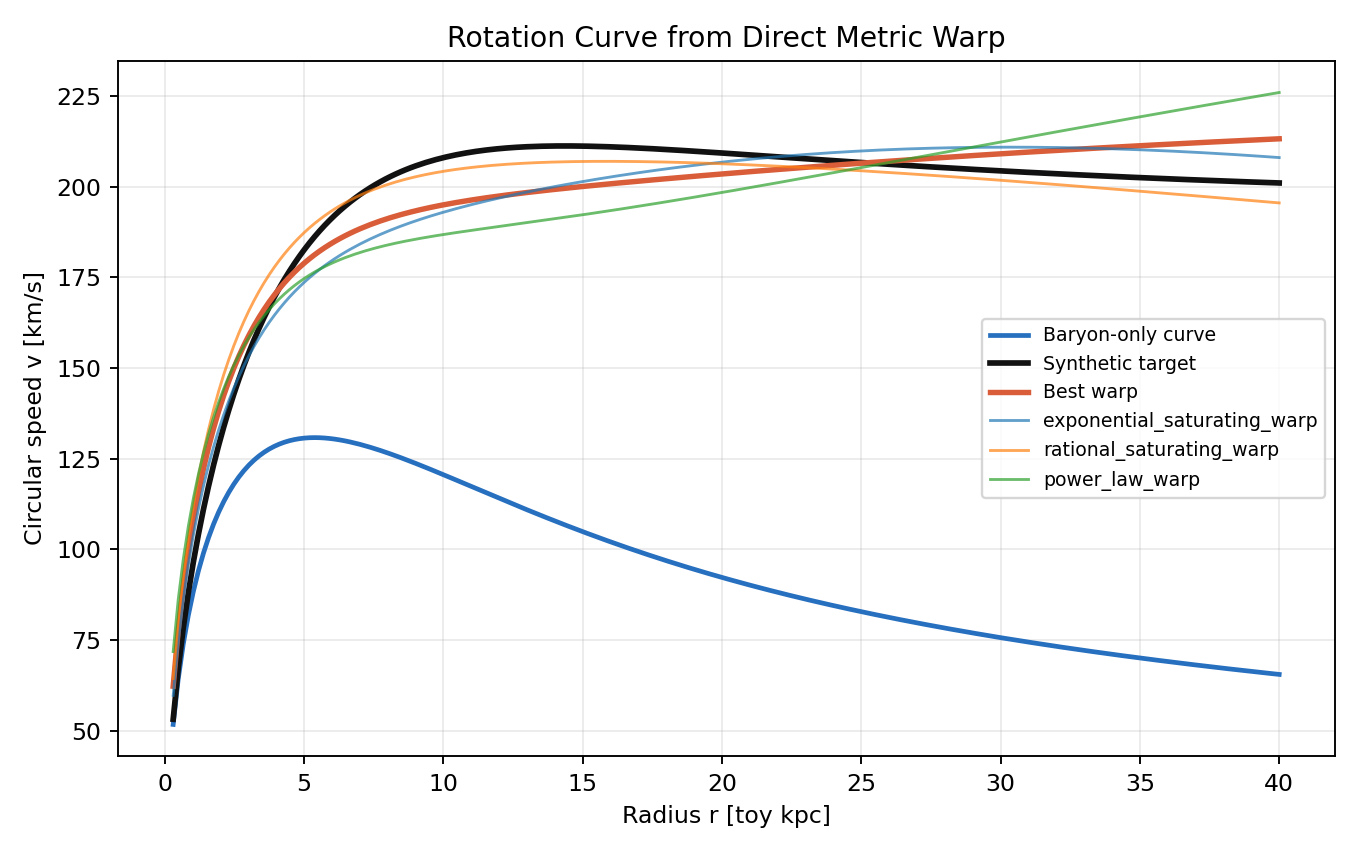
\includegraphics[width=\linewidth]{warp_rotation_fit.png}
\end{minipage}\hfill
\begin{minipage}{0.49\linewidth}
\centering
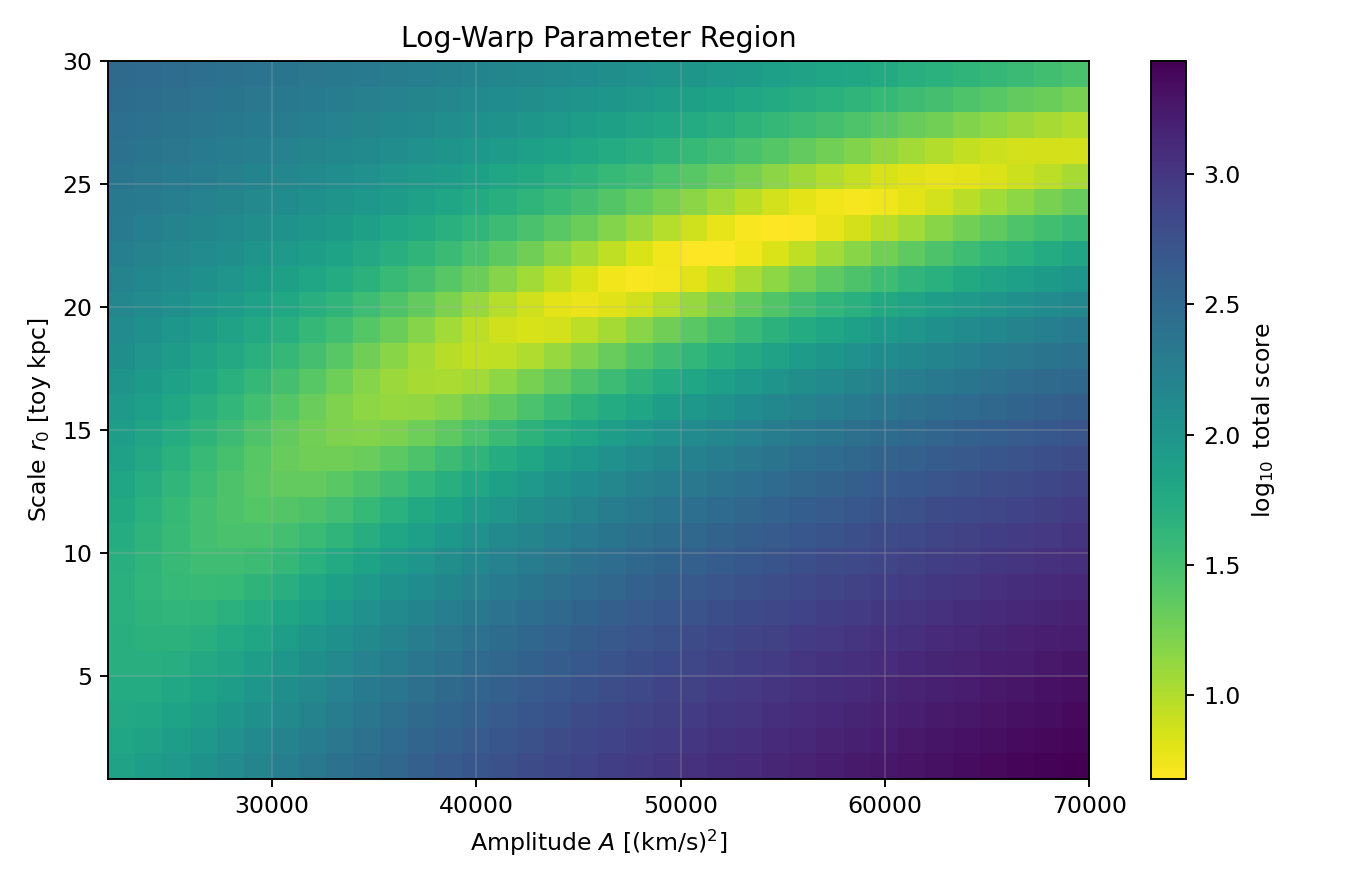
\includegraphics[width=\linewidth]{warp_log_parameter_heatmap.png}
\end{minipage}
\caption{Weak-field warp search. Left: the best direct metric perturbation reproduces the synthetic flat rotation curve. Right: the logarithmic warp family contains a broad low-score region, reflecting that flat circular speed requires $\dd\delta\Phi/\dd r\sim1/r$ over the outer radial range.}
\label{fig:warp}
\end{figure}

\section{Results}

The best-ranked candidate was a no-slip logarithmic warp,
\begin{equation}
\delta\Phi
=
A\log(1+r/r_0),
\qquad
A\simeq5.49\times10^4\ {\rm km^2\,s^{-2}},
\quad
r_0\simeq13.4\ {\rm kpc}.
\end{equation}
It achieved total score $4.79$, rotation weighted MSE $2.08$, lensing-proxy MSE $0.118$, outer flatness metric $0.0117$, and $\max|\Phi|/c^2\simeq1.4\times10^{-6}$. The left panel of Fig.~\ref{fig:warp} shows that this warp reproduces the synthetic target curve while preserving the baryon-only baseline as the comparison. The right panel explains why this is not an isolated numerical accident: the logarithmic family contains a broad low-score region. Exponential and rational saturating warps also fit reasonably, but the logarithmic family gave the best balance of rotation fit, lensing proxy, smoothness, and simplicity. Gaussian bump warps performed poorly because their derivatives are localized and sign-changing.

This is the expected result, but recovered without naming a physical source. A flat outer rotation curve implies $v^2\simeq{\rm const.}$, hence
\begin{equation}
\frac{\dd\delta\Phi}{\dd r}
\simeq
\frac{v_f^2}{r},
\qquad
\delta\Phi
\simeq
v_f^2\log r.
\end{equation}
The effective density proxy is extended rather than localized, and the successful warps remain well inside the weak-field regime. This is the role of the left panel of Fig.~\ref{fig:effective}: it translates the best potential perturbation into the cumulative effective mass and density proxy, making clear what kind of source structure the residual would require if interpreted on the right-hand side of Einstein's equation.

\begin{figure}[t]
\centering
\begin{minipage}{0.49\linewidth}
\centering
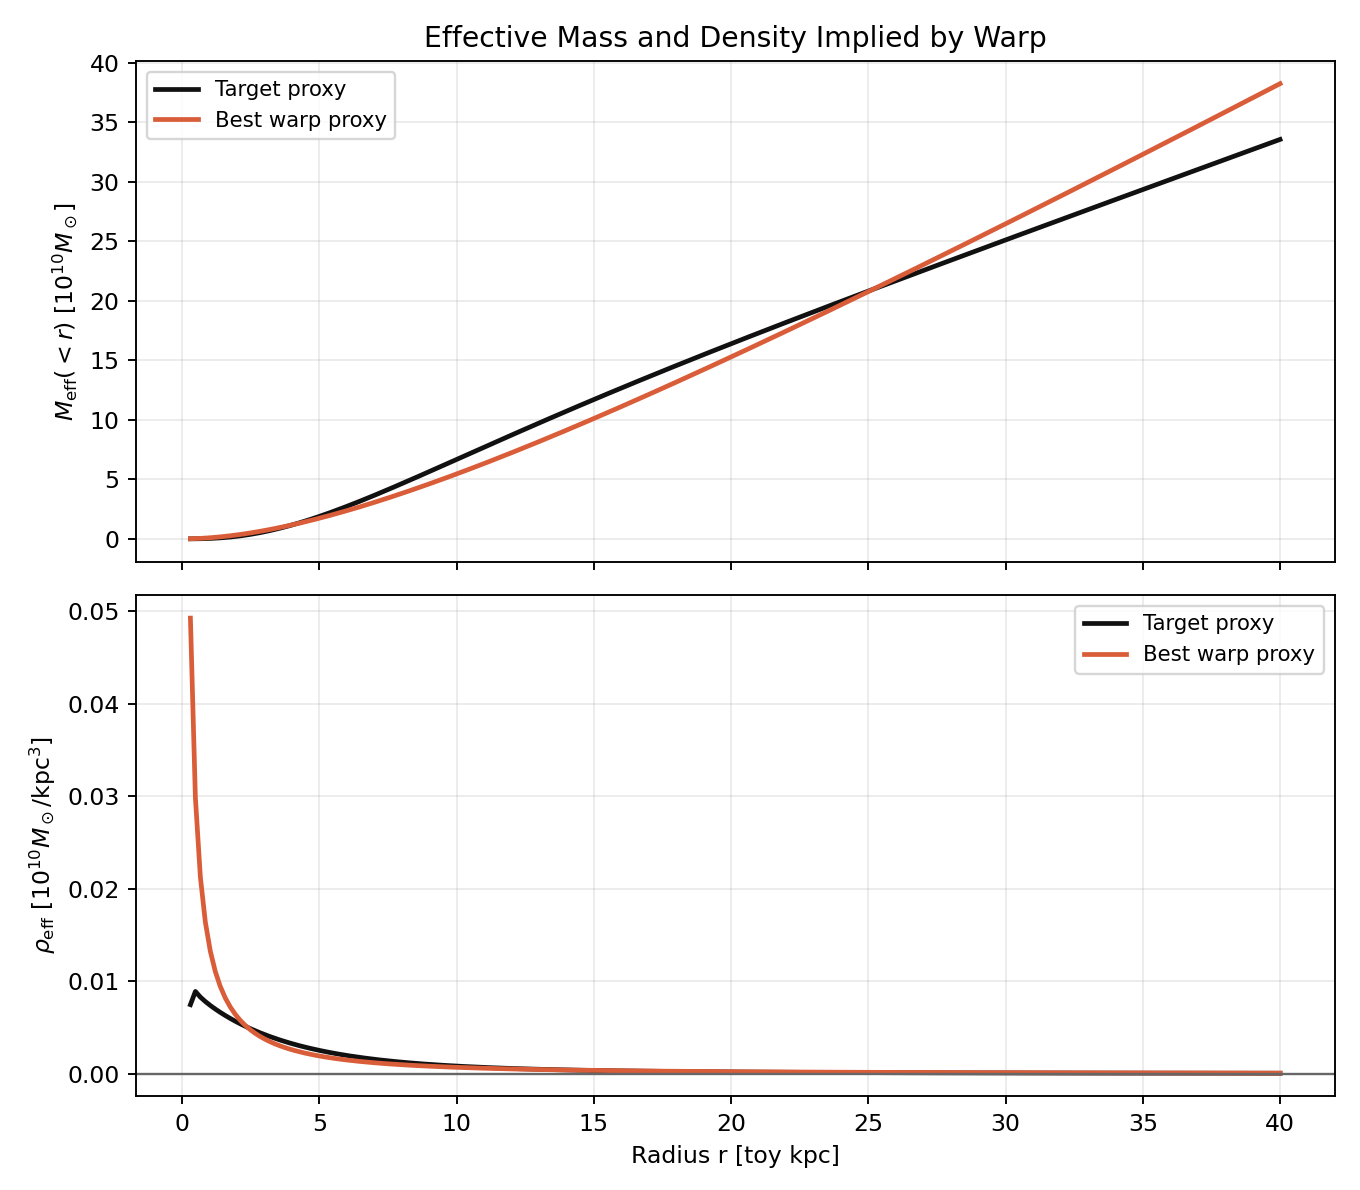
\includegraphics[width=\linewidth]{warp_effective_profiles.png}
\end{minipage}\hfill
\begin{minipage}{0.49\linewidth}
\centering
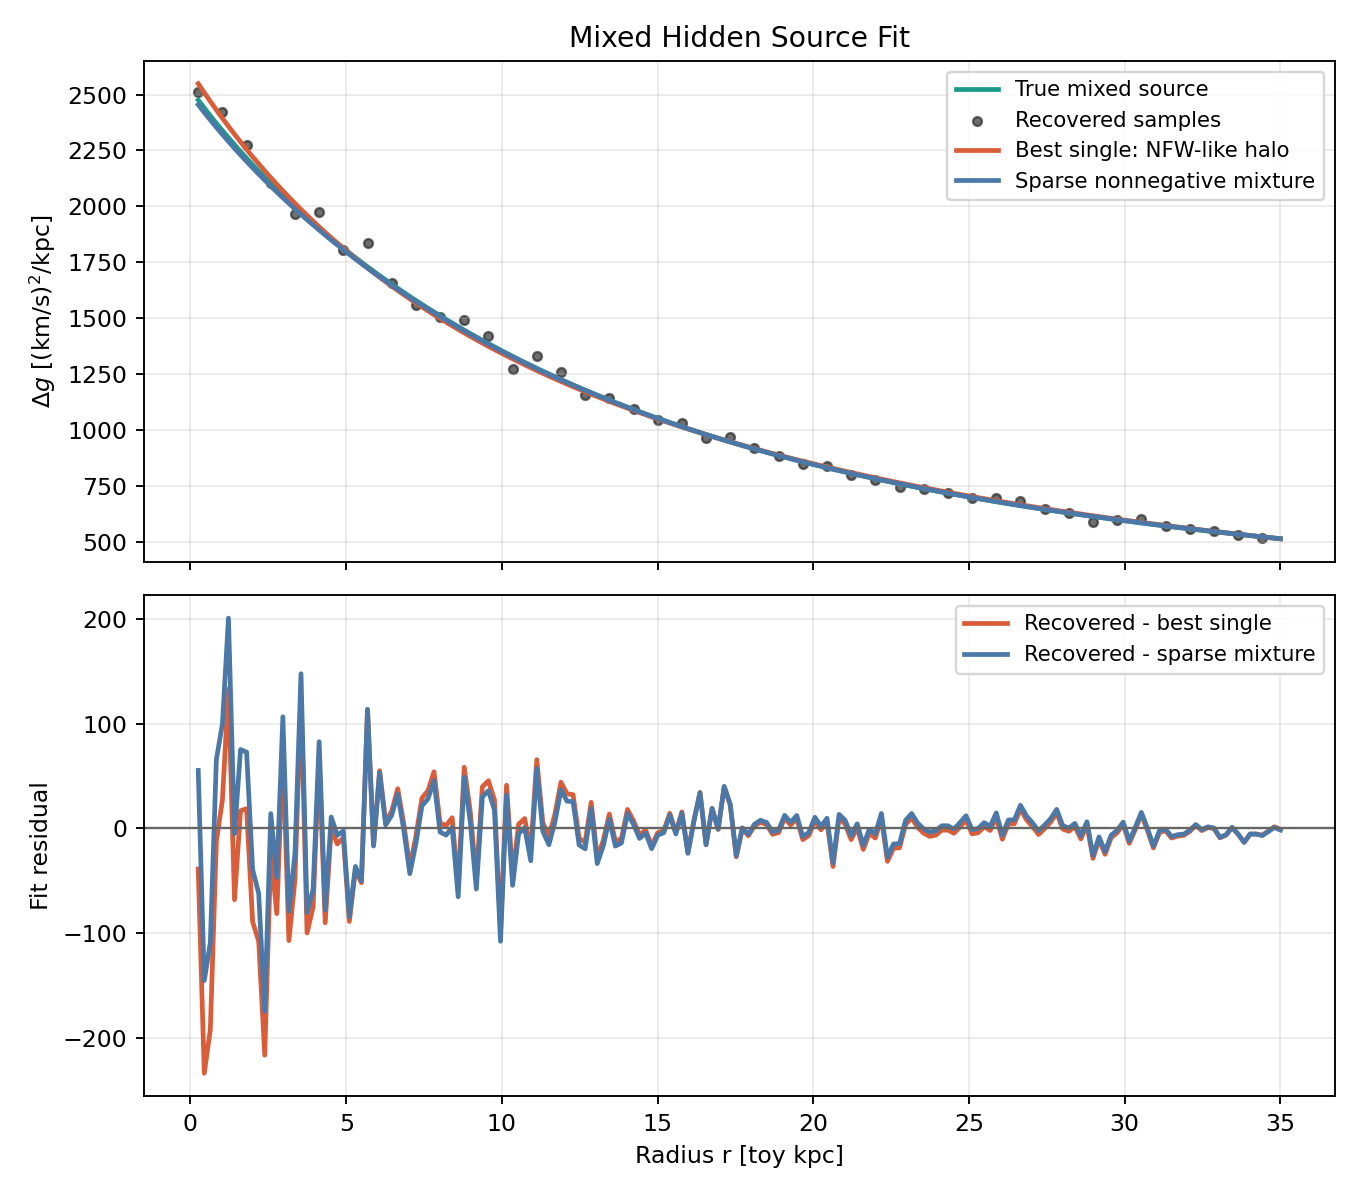
\includegraphics[width=\linewidth]{mixed_source_fit.png}
\end{minipage}
\caption{Effective structure and named-generator comparison. Left: the best warp implies an extended monotone effective mass and mostly nonnegative density proxy in the spherical toy inversion. Right: in the separate named-generator scaffold, a sparse two-term mixture fits a mixed synthetic residual better than any single named family, illustrating that residual decomposition is itself degenerate.}
\label{fig:effective}
\end{figure}

The named-generator scaffold reinforces the degeneracy. For a synthetic mixed source, the sparse nonnegative mixture had weighted MSE $0.575$ and BIC-like score $-89.25$, beating the best single family, an NFW-like profile with weighted MSE $0.611$ and BIC-like score $-78.28$. The selected terms were an NFW-shaped component and a MOND-shaped acceleration relation. The right panel of Fig.~\ref{fig:effective} is therefore not presented as evidence for either named model; it is a warning that rotation data can absorb multiple latent mechanisms into similar residual curves.

\section{Interpretation, Limitations, and Next Steps}

The narrative arc is now: observations define a geometric residual; weak-field dynamics reduce part of it to $\Delta g=\dd\delta\Phi/\dd r$; a theory-agnostic search over $\delta\Phi$ and $\delta\Psi$ identifies which spacetime warps reproduce the residual; only then should one ask what physical generator could produce such a warp. Figure~\ref{fig:warp} supports the first computational step, moving from rotation residual to direct metric-warp search. Figure~\ref{fig:effective} supports the second step, translating the successful warp into an effective source structure and showing why named physical decompositions remain degenerate. In the toy flat-curve case, the residual asks for a smooth, long-range perturbation close to logarithmic growth. The named-generator fit then shows that several physical stories can mimic parts of the same field structure.

Several caveats are essential. The units and data are synthetic. The inversion is radial and spherical, not a disk-galaxy mass model. No full Einstein tensor is computed. The lensing/slip observable is conceptual, not physical lensing. Coordinate and gauge issues are suppressed by the chosen ansatz. The search does not discover particles, fields, or modified equations; it only maps which weak-field perturbations satisfy a chosen set of diagnostics.

The most promising next steps are to fit real SPARC-like rotation curves \citep{Lelli2016}; replace the spherical proxy with disk geometry; compute full metric-perturbation curvature diagnostics; use automatic differentiation over metric ansatz families; enforce conservation,
\begin{equation}
\nabla^\mu T^{\rm eff}_{\mu\nu}=0;
\end{equation}
jointly fit rotation and lensing; and classify learned warp families across galaxy populations before assigning physical explanations.

\section{Compact Thesis}

The missing-mass problem can be summarized as
\begin{equation}
\boxed{
G_{\mu\nu}[g^{\rm obs}]
-
G_{\mu\nu}[g^{\rm bar}]
=
\cG \Tmiss,
}
\end{equation}
with
\begin{equation}
\boxed{
\Tmiss
=
\sum_k T^{(k)}_{\mu\nu}.
}
\end{equation}
In the weak-field galaxy limit,
\begin{equation}
\boxed{
\Delta g(r)
=
\frac{v_{\rm obs}^2(r)-v_{\rm bar}^2(r)}{r},
\qquad
\rho_{\rm miss}
=
\frac{1}{4\pi G}\nabla^2\Delta\Phi.
}
\end{equation}
The more primitive computational search is
\begin{equation}
\boxed{
g_{\mu\nu}^{\rm trial}
=
g_{\mu\nu}^{\rm bar}
+
h_{\mu\nu}(\theta),
}
\end{equation}
where $h_{\mu\nu}(\theta)$ is explored directly before it is interpreted as dark matter, modified gravity, baryonic error, or systematics. In one sentence: the missing-mass problem can be studied as an inverse problem over geometric residuals--infer the simplest physically valid generator, or mixture of generators, whose induced curvature residual matches observations across probes.

\begingroup\small
\begin{thebibliography}{9}

\bibitem[Rubin et~al.(1980)]{Rubin1980}
Rubin, V. C., Ford, W. K., Jr., \& Thonnard, N. (1980).
Rotational properties of 21 Sc galaxies with a large range of luminosities and radii.
\emph{The Astrophysical Journal}, 238, 471--487.
\href{https://doi.org/10.1086/158003}{doi:10.1086/158003}.

\bibitem[Lelli et~al.(2016)]{Lelli2016}
Lelli, F., McGaugh, S. S., \& Schombert, J. M. (2016).
SPARC: Mass models for 175 disk galaxies with Spitzer photometry and accurate rotation curves.
\emph{The Astronomical Journal}, 152, 157.
\href{https://doi.org/10.3847/0004-6256/152/6/157}{doi:10.3847/0004-6256/152/6/157}.

\bibitem[McGaugh et~al.(2016)]{McGaugh2016}
McGaugh, S. S., Lelli, F., \& Schombert, J. M. (2016).
The radial acceleration relation in rotationally supported galaxies.
\emph{Physical Review Letters}, 117, 201101.
\href{https://doi.org/10.1103/PhysRevLett.117.201101}{doi:10.1103/PhysRevLett.117.201101}.

\bibitem[Bertone \& Hooper(2018)]{Bertone2018}
Bertone, G., \& Hooper, D. (2018).
History of dark matter.
\emph{Reviews of Modern Physics}, 90, 045002.
\href{https://doi.org/10.1103/RevModPhys.90.045002}{doi:10.1103/RevModPhys.90.045002}.

\bibitem[Mistele et~al.(2024)]{Mistele2024}
Mistele, T., McGaugh, S., Lelli, F., Schombert, J., \& Li, P. (2024).
Indefinitely flat circular velocities and the baryonic Tully-Fisher relation from weak lensing.
\emph{The Astrophysical Journal Letters}, 969, L3.
\href{https://doi.org/10.3847/2041-8213/ad54b0}{doi:10.3847/2041-8213/ad54b0}.

\end{thebibliography}
\endgroup

\end{document}
